\subsection{Valutazioni}
Nel caso del task di Named Entity Recognition, i risultati presentano una notevole differenza tra le performance ottenute con i dataset in lingua inglese e in lingua italiana. Infatti, si passa da un F1-score dell'87\% con BERT Base nel primo caso, ad un 60\% con il modello corrispettivo per la lingua italiana. Il risultato per l'inglese non raggiunge lo stato dell'arte\footnote{Risultati CoNLL 2003 (English): \href{https://paperswithcode.com/sota/named-entity-recognition-ner-on-conll-2003}{https://paperswithcode.com/sota/named-entity-recognition-ner-on-conll-2003}}, ma non si distacca eccessivamente dalle altre soluzioni al momento disponibili. Drastico è il calo che si ha con la lingua italiana, dove il modello sbaglia eccessivamente. Da quanto si evince dei risultati mostrati sul sito di \textit{evalita}\footnote{Risultati evalita 2009: \href{https://www.evalita.it/evalita-2009/results/}{https://www.evalita.it/evalita-2009/results/}}, le soluzioni per questo task raggiungono anche valori di F1-score pari all'82\%, ovvero circa il 20\% in più del modello studiato in questa tesi. I risultati peggiori, come si legge dal classification report, si incontrano nei casi dei tag che identificano \textit{entità geo-politiche (GPE)} e \textit{organizzazioni (ORG)}.
\begin{figure}[ht!]
    \centering
    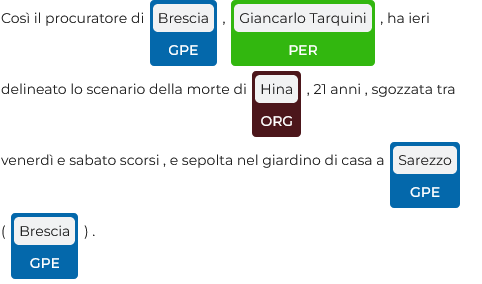
\includegraphics[width=0.8\textwidth]{img/errori_ner_ita/errore1.png}
    \caption{Named Entity Recognition per l'italiano - Errore 1}
    \label{fig:ner_errore1}
\end{figure}
\begin{figure}[ht!]
    \centering
    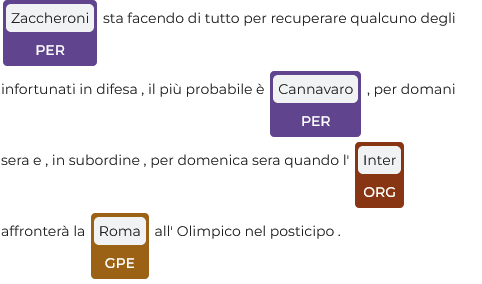
\includegraphics[width=0.8\textwidth]{img/errori_ner_ita/errore2.png}
    \caption{Named Entity Recognition per l'italiano - Errore 2}
    \label{fig:ner_errore2}
\end{figure} \newpage
Osservando la figura \ref{fig:ner_errore1}, si nota come nomi poco frequenti in Italia (in questo caso \textit{Hina}), non vengono interpretati come riferimenti a persone, ma ad altre entità (in questo caso \textit{organizzazione (ORG)}).
Inoltre, il modello fatica a distinguere le ambiguità che si presentano quando un'entità che solitamente è utilizzata con un significato, si presenta nella frase con un'altra accezione. Facendo riferimento all'immagine \ref{fig:ner_errore2}, il concetto di \textit{Roma} come associazione sportiva, e quindi \textit{organizzazione}, viene confuso con il significato di \textit{Roma} intesa come la città capitale d'Italia. La parola è stata pertanto classificata come entità \textit{geo-politica}.
 

Un'ulteriore differenza tra i dati ottenuti dai due dataset, si ha con l'accuratezza raggiunta dai modelli. Anche se di poco, BERT performa meglio di GloVe nella lingua inglese (86.5\% il primo, 85,8\% il secondo), mentre per la lingua italiana, GloVe riconosce leggermente meglio le ambiguità rispetto alla controparte (65\% per GloVe, 60,5\% BERT).\\
\\
Passando al problema di Text Classification, sia il componente UniversalSentenceEncoder sia il BertSentenceEmbedding, riportano ottimi risultati in termini di accuratezza, raggiungendo entrambi l'89\%. La differenza sostanziale si nota nei tempi di esecuzione, nei quali l'\verb|UniversalSentenceEncoder| risulta essere decine di volte più veloce. Pertanto, a parità di risultati, USE è l'alternativa che offre il miglior rapporto tra l'accuracy e i tempi di esecuzione sui dataset utilizzati.\\
\\
É facilmente osservabile che, all'aumentare della dimensione del sistema distribuito, e quindi degli esecutori, Spark NLP migliora di gran lunga le sue prestazioni. La differenza si nota in particolar modo con BERT, dove non si ottiene ancora un risultato in tempi competitivi ma, con l'aggiunta di un nodo worker, il tempo di esecuzione si dimezza. Questo denota una buona distribuzione del carico di lavoro tra i nodi dovuta ad un'equa suddivisione dei jobs tra i vari esecutori. 

In sistemi che utilizzano frequentemente centinaia se non migliaia di nodi, Spark NLP può offrire predizioni accurate in tempi contenuti.